\thispagestyle{duongvaotoanhocnone}
\pagestyle{duongvaotoanhoc}
\everymath{\color{duongvaotoanhoc}}
\graphicspath{{../duongvaotoanhoc/pic/}}
\blfootnote{$^1$\color{duongvaotoanhoc}Images des Mathématiques, http://images.math.cnrs.fr/Les-tresses-de-la-topologie-a-la-cryptographie.html.}
\blfootnote{$^2$\color{duongvaotoanhoc}Giáo sư, Đại học Bourgogne, Pháp.}
\blfootnote{$^3$\color{duongvaotoanhoc}Hiệu đính bởi Étienne Ghys.}
\begingroup
\AddToShipoutPicture*{\put(0,616){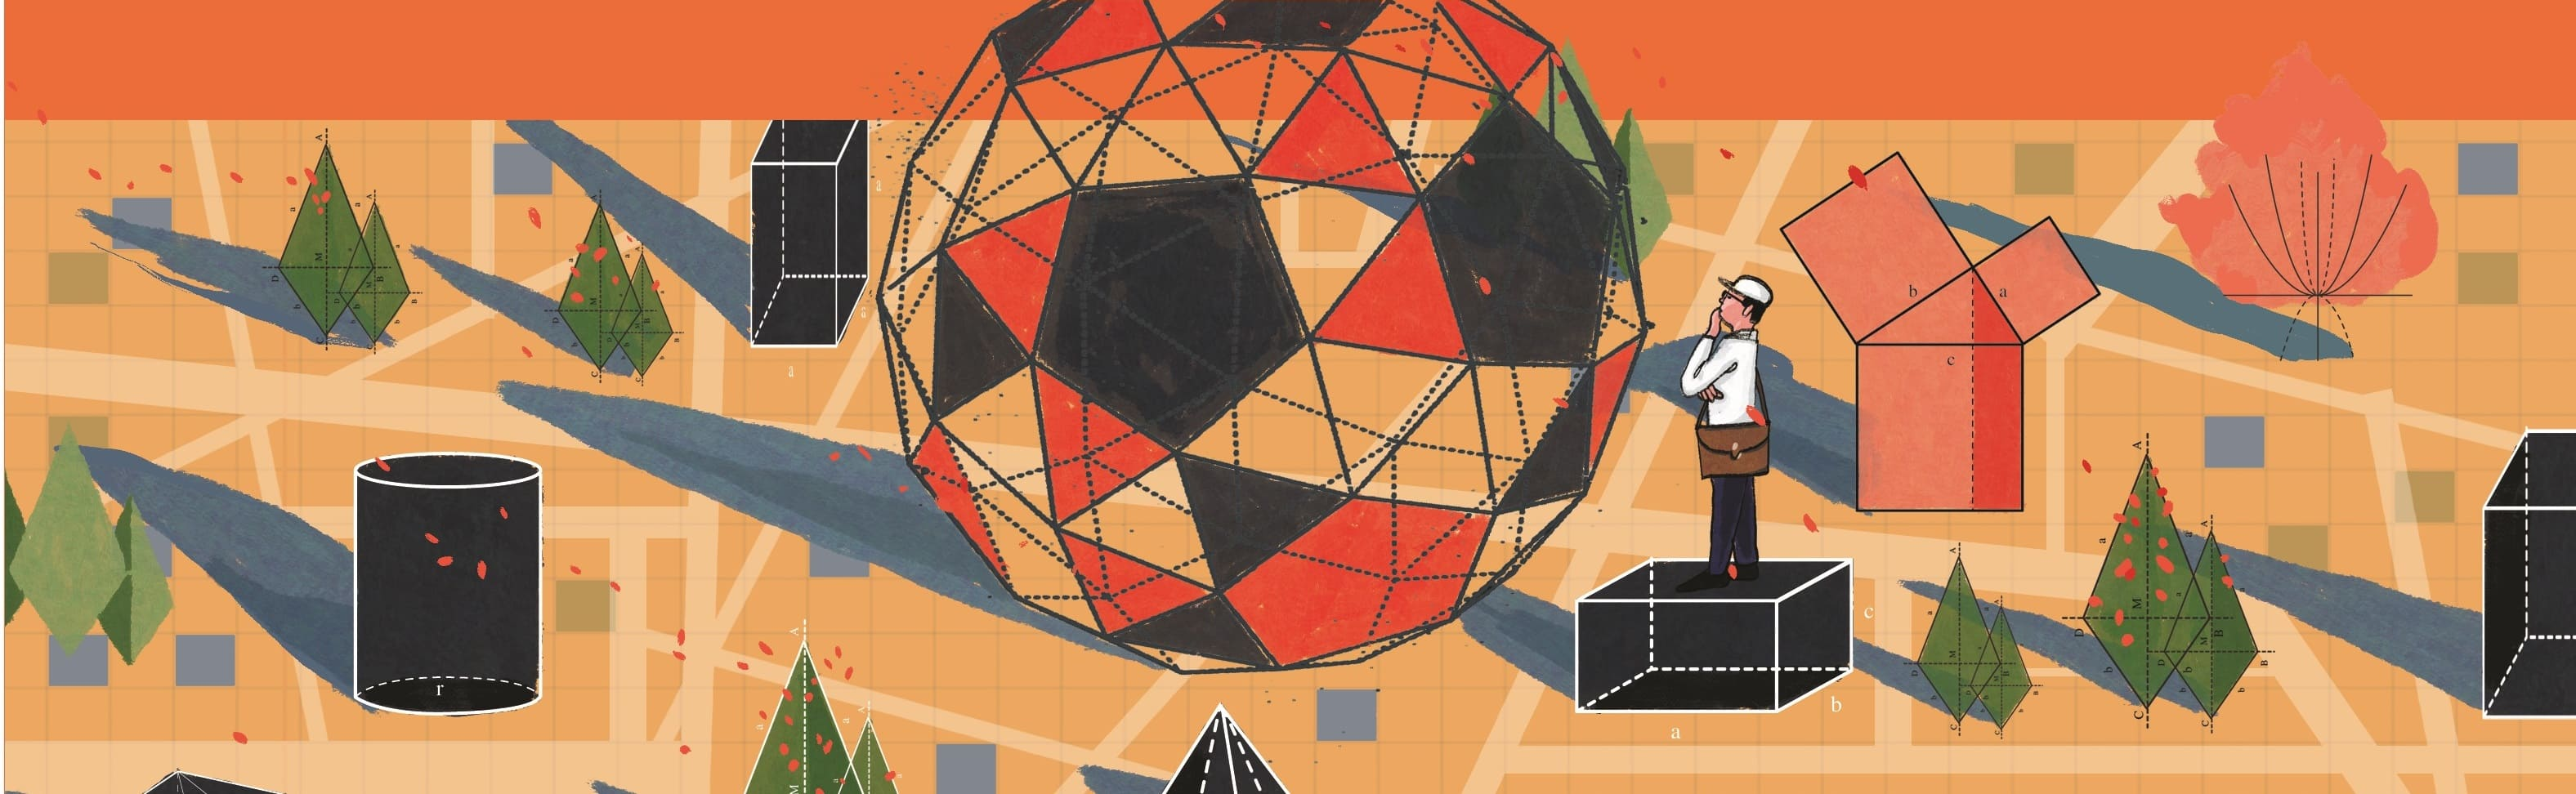
\includegraphics[width=19.3cm]{../bannerduongvao}}}
\AddToShipoutPicture*{\put(82,555){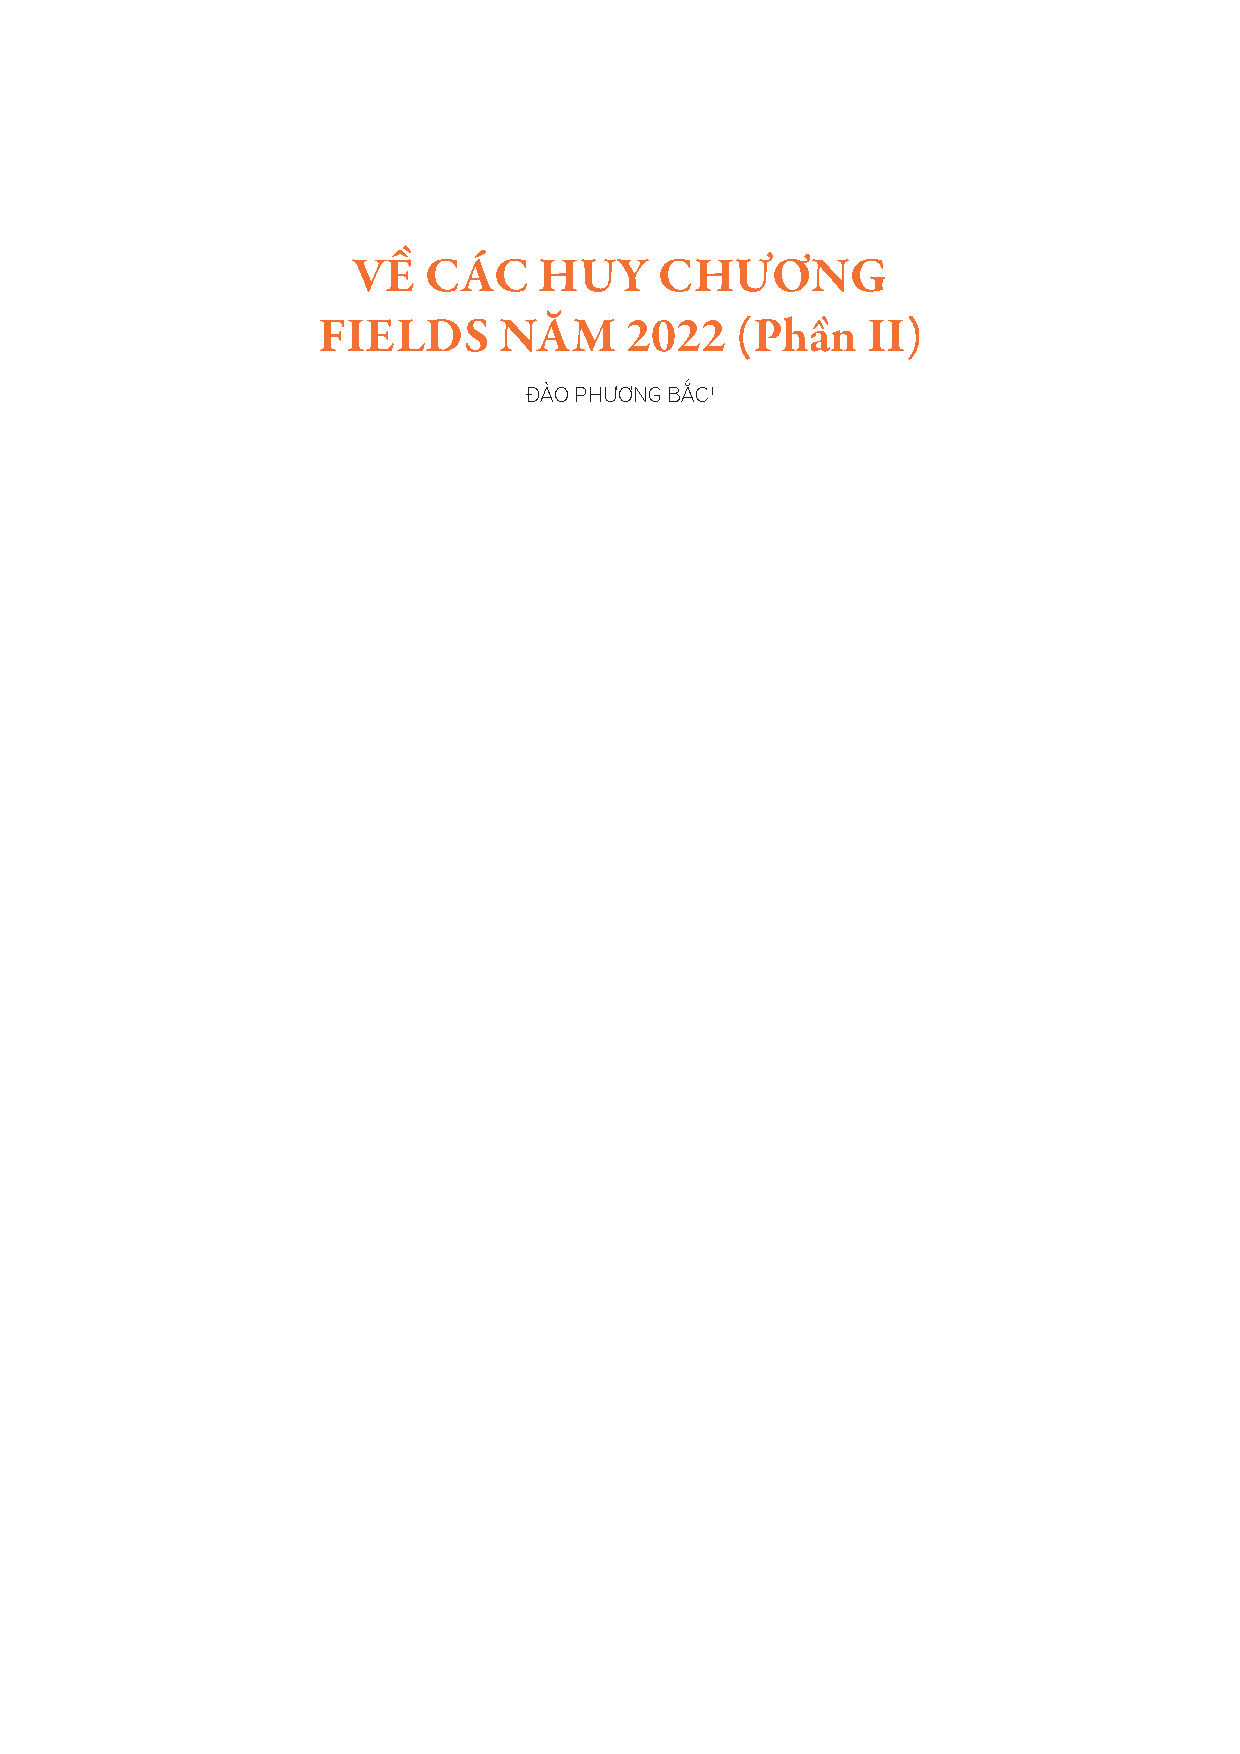
\includegraphics[scale=1]{../tieude.pdf}}}
\centering
\endgroup

\vspace*{150pt}

\tikzstyle{start} = [rectangle, rounded corners, minimum height=1cm,text centered, draw=black, fill=red!30]

\tikzstyle{end} = [rectangle, rounded corners, minimum height=1cm,text centered, draw=black, fill=blue!30]

\tikzstyle{mid} = [rectangle, rounded corners, minimum height=1cm,text centered, draw=black, fill=green!30]

\begin{multicols}{2}	
	$\pmb{1.}$ \textbf{\color{duongvaotoanhoc}Mở đầu}
	\vskip 0.1cm
	\textbf{\color{duongvaotoanhoc}Từ dải bện...}
	\vskip 0.1cm
	Dải bện đã tồn tại từ nhiều thế kỷ và được sử dụng khắp nơi vì mục đích trang trí cũng như trong đời sống, chẳng hạn trong sản xuất dây thừng hoặc dây cáp. Một dải bện có thể gồm ba sợi, hay cọng, được tết với nhau: cọng trái được vắt qua cọng giữa, rồi đến cọng phải, rồi lại cọng trái, rồi lại cọng phải, cứ thế lặp đi lặp lại (xem Hình $1$). Nhưng ``dải bện" cũng được dùng để chỉ mọi sự đan hay tết của nhiều cọng dây theo một cách nhất định. Trong Hình $2$ và Hình $3$ là một số thí dụ về các dải bện trang trí.
	\begin{figure}[H]
		\vspace*{-5pt}
		\centering
		\captionsetup{labelformat= empty, justification=centering}
		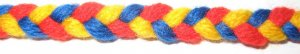
\includegraphics[width= 0.7\linewidth]{fig_01}
		\caption{\small\textit{\color{duongvaotoanhoc}Hình $1$. Dải bện cổ điển với ba cọng dây.}}
		\vspace*{-10pt}
	\end{figure}
	\begin{figure}[H]
		\vspace*{-10pt}
		\centering
		\captionsetup{labelformat= empty, justification=centering}
		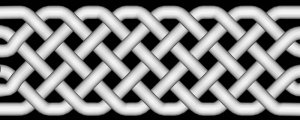
\includegraphics[width= 0.7\linewidth]{fig_02}
		\caption{\small\textit{\color{duongvaotoanhoc}Hình $2$. Một dải bện trang trí.}}
		\vspace*{-10pt}
	\end{figure}
	\textbf{\color{duongvaotoanhoc}... đến lý thuyết bện}
	\vskip 0.1cm
	Các nhà toán học mô tả các dải bện bằng các mô hình trừu tượng, những đối tượng trung tâm của một lý thuyết toán học có tên ``lý thuyết bện". Lý thuyết này đóng một vai trò trung tâm trong toán học và len lỏi vào trong nhiều ngành toán học, cũng như các khoa học khác như vật lý, sinh học, tin học và mật~mã.
	\begin{figure}[H]
		\vspace*{-5pt}
		\centering
		\captionsetup{labelformat= empty, justification=centering}
		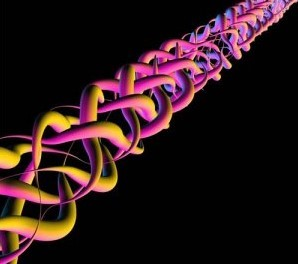
\includegraphics[width= 0.65\linewidth]{fig_03a}
		\caption{\small\textit{\color{duongvaotoanhoc}Hình $3$. Một dải bện trang trí khác.}}
		\vspace*{-10pt}
	\end{figure}
	%	\vskip 0.1cm
	Bài viết này nhằm đem đến cho độc giả không làm toán một cái nhìn bao quát về lý thuyết bện. Chúng tôi sẽ đưa ra định nghĩa bện trong toán học, sau đó minh họa ứng dụng của chúng trong ba lĩnh vực: lý thuyết nút (toán học), lý thuyết thuật toán (toán học và tin học), và lý thuyết mật mã (toán học, tin học và viễn thông). Ngoài ra, chúng còn nhiều ứng dụng và tương tác qua lại khác với các phần khác của toán học, và với cả, chẳng hạn, vật lý thiên văn. Thực vậy, các đường từ trường trong khí quyển Mặt Trời tạo thành các dải bện mà độ phức tạp có liên hệ trực tiếp đến cường độ của từ trường.
	\vskip 0.1cm
	$\pmb{2.}$ \textbf{\color{duongvaotoanhoc}Dải bện trong toán học}
	\vskip 0.1cm
	\textbf{\color{duongvaotoanhoc}Thế nào là một dải bện trong toán học?}
	\vskip 0.1cm
	\textit{Lý thuyết bện} tách khái niệm bện khỏi những dải bện mà ta vẫn thường nghĩ đến. Trước tiên, ta cố định một số tự nhiên $n$. Để tiện trình bày, ta sẽ lấy $n = 4$, mặc dù tất cả những gì được mô tả tiếp theo đây đúng với mọi giá trị của $n$. Chúng ta lấy hai tập hợp, mỗi tập hợp có $4$ vật (chẳng hạn những cái đinh) và để chúng trên bàn thành hai hàng dọc đối diện nhau (các chấm đen trong hình). Sử dụng bốn sợi dây, mà ta gọi là cọng, ta nối mỗi vật trong tập hợp thứ nhất với một vật trong tập hợp thứ hai. Một kết nối như vậy được gọi là một dải bện. Các cọng có thể vắt qua nhau, nhưng không được vòng ngược lại. Kết nối trong Hình $5$ không phải là một dải bện (theo nghĩa toán học).
	\begin{figure}[H]
		\vspace*{-10pt}
		\centering
		\captionsetup{labelformat= empty, justification=centering}
		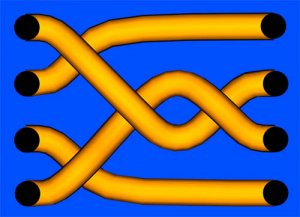
\includegraphics[width= 0.465\linewidth]{fig_04}\quad
		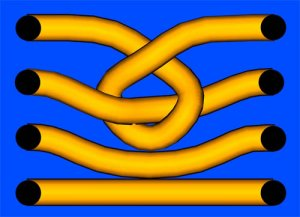
\includegraphics[width= 0.465\linewidth]{fig_05}
		\caption{\small\textit{\color{duongvaotoanhoc}Hình $4$. Một dải bện \hspace*{18pt} Hình $5$. Đây không \hspace*{10pt}\\
				\hspace*{20pt}toán học.\hspace*{45pt} phải một dải bện. }}
		\vspace*{-10pt}
	\end{figure}
	\begin{figure}[H]
		\vspace*{-10pt}
		\centering
		\captionsetup{labelformat= empty, justification=centering}
		
		\caption{\small\textit{\color{duongvaotoanhoc}}}
		\vspace*{-10pt}
	\end{figure}	
	Trong Hình $6$ là hai dải bện khác nhau. Trong khi đó, hai dải bện trong Hình $7$ là giống nhau, vì chúng có thể nhận được từ nhau bằng cách ``xê dịch" các cọng.
	\begin{figure}[H]
		\vspace*{-10pt}
		\centering
		\captionsetup{labelformat= empty, justification=centering}
		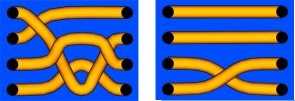
\includegraphics[width= 1\linewidth]{fig_06}
		\caption{\small\textit{\color{duongvaotoanhoc}Hình $6$. Hai dải bện khác nhau.}}
		\vspace*{-10pt}
	\end{figure}
	\begin{figure}[H]
		\vspace*{-10pt}
		\centering
		\captionsetup{labelformat= empty, justification=centering}
		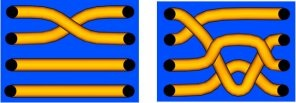
\includegraphics[width= 0.97\linewidth]{fig_07}
		\caption{\small\textit{\color{duongvaotoanhoc}Hình $7$. Hai dải bện giống nhau.}}
		\vspace*{-10pt}
	\end{figure}
	Một dải bện cũng có thể được coi như một chuỗi các đường đi của $4$ hạt không gặp nhau. Ở đây, tập hợp các điểm xuất phát trùng với tập hợp các điểm đến. Thí dụ, các quỹ đạo của $4$ hạt được thể hiện ở nửa trên của Hình $8$ tương ứng với dải bện ở nửa dưới. Một cách nôm na, các dải bện có thể được xem như những điệu nhảy mà ở đó, mỗi vũ công kết thúc ở vị trí của một vũ công khác.
	\begin{figure}[H]
		\vspace*{-5pt}
		\centering
		\captionsetup{labelformat= empty, justification=centering}
		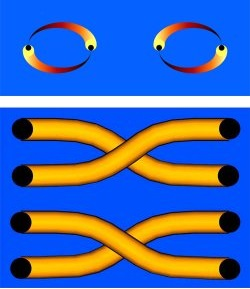
\includegraphics[width= 0.475\linewidth]{fig_08}
		\caption{\small\textit{\color{duongvaotoanhoc}Hình $8$. Hai cách nhìn của cùng một dải bện.}}
		\vspace*{-10pt}
	\end{figure}
	\vskip 0.1cm
	\PIbox{
		\begin{figure}[H]
			\vspace*{-10pt}
			\centering
			\captionsetup{labelformat= empty, justification=centering}
			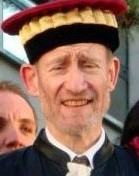
\includegraphics[width= 1\linewidth]{fig_Dehornoy}
			\caption{\small\textit{\color{duongvaotoanhoc}Patrick Dehornoy.}}
			\vspace*{-10pt}
		\end{figure}
		Patrick Dehornoy ($1952-2019$) là nhà toán học Pháp được biết đến vì những công trình trong lý thuyết tập hợp và lý thuyết bện. Ông nguyên là giáo sư tại Đại học Caen và là thành viên kỳ cựu của Viện Đại học Pháp (Institut Universitaire de France). Ông là người sáng lập nhóm nghiên cứu GDR TRESSES, nơi tập trung các nghiên cứu về lý thuyết bện của nước Pháp.
	}
	\textbf{\color{duongvaotoanhoc}Ghép các dải bện}
	\vskip 0.05cm
	Từ hai dải bện $\alpha$ và $\beta$, ta có thể xây dựng một phép thứ ba, ký hiệu là $\alpha \beta$ và được gọi là dải bện hợp thành của $\alpha$ và $\beta$, bằng cách ghép chúng với nhau. Trong Hình $9$ là hai dải bện (bên trên) và hợp thành của chúng (bên dưới).
	\begin{figure}[H]
		\vspace*{-5pt}
		\centering
		\captionsetup{labelformat= empty, justification=centering}
		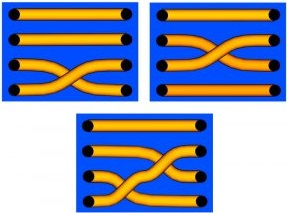
\includegraphics[width= 0.97\linewidth]{fig_09}
		\caption{\small\textit{\color{duongvaotoanhoc}Hình $9$. Hợp thành của hai dải bện.}}
		\vspace*{-5pt}
	\end{figure}
	Một thí dụ khác về phép hợp thành được minh họa trong Hình $10$.
	\begin{figure}[H]
		\vspace*{-5pt}
		\centering
		\captionsetup{labelformat= empty, justification=centering}
		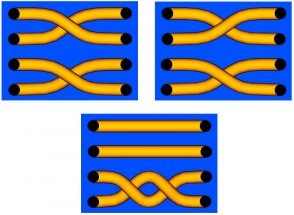
\includegraphics[width= 0.97\linewidth]{fig_10}
		\caption{\small\textit{\color{duongvaotoanhoc}Hình $10$. Hợp thành của hai dải bện khác.}}
		\vspace*{-10pt}
	\end{figure}
	Bạn đọc có kinh nghiệm hẳn đã để ý rằng dải bện $\alpha \beta$ có thể khác với dải bện $\beta \alpha$: điều này xảy ra với thí dụ trong Hình $9$, nhưng không đúng với thí dụ trong Hình $10$.
	\vskip 0.1cm
	Dải bện trong Hình $11$ được gọi là \textit{dải bện tầm thường}. Dễ thấy hợp của một dải bện $\alpha$ bất kỳ với dải bện tầm thường, từ bên trái hay từ bên phải, vẫn là $\alpha$.
	\begin{figure}[H]
		\vspace*{-5pt}
		\centering
		\captionsetup{labelformat= empty, justification=centering}
		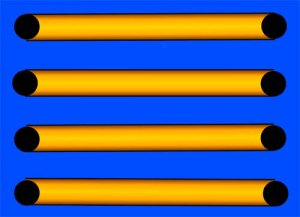
\includegraphics[width= 0.47\linewidth]{fig_11}
		\caption{\small\textit{\color{duongvaotoanhoc}Hình $11$. Dải bện tầm thường.}}
		\vspace*{-10pt}
	\end{figure}
	Nếu ta đặt một tấm gương vuông góc với mặt bàn ở cạnh hàng đinh thứ hai, ảnh phản chiếu trong gương của dải bện $\alpha$ được gọi là dải bện đối xứng của $\alpha$ (xem Hình $12$). Hợp thành của một dải bện với dải bện đối xứng của nó là dải bện tầm thường. Bạn đọc có thể dễ dàng kiểm chứng với thí dụ trong Hình $12$.
	\begin{figure}[H]
		\vspace*{-5pt}
		\centering
		\captionsetup{labelformat= empty, justification=centering}
		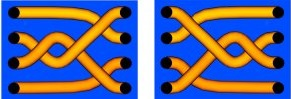
\includegraphics[width= 0.97\linewidth]{fig_12}
		\caption{\small\textit{\color{duongvaotoanhoc}Hình $12$. Một dải bện và dải bện đối xứng của~nó.}}
		\vspace*{-5pt}
	\end{figure}
	\textbf{\color{duongvaotoanhoc}Từ dải bện đến nhóm bện}
	\vskip 0.1cm
	Những dải bện, như chúng ta vừa định nghĩa, cùng với phép hợp thành tạo thành cái mà các nhà toán học gọi là \textit{nhóm bện}. Chúng ta có một nhóm bện [gồm các dải bện có] hai cọng, một nhóm bện ba cọng, v.v. Nhóm bện một cọng chỉ gồm dải bện tầm thường, vì một cọng thì không thể được bện, dù nó có thể được buộc thắt nút (xem Hình $13$).
	\begin{figure}[H]
		\vspace*{-5pt}
		\centering
		\captionsetup{labelformat= empty, justification=centering}
		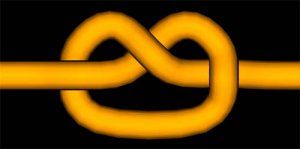
\includegraphics[width= 0.6\linewidth]{fig_13}
		\caption{\small\textit{\color{duongvaotoanhoc}Hình $13$. Cọng buộc thắt nút.}}
		\vspace*{-10pt}
	\end{figure}
	Phép hợp thành của các dải bện tuân theo một số quy tắc mà đối với các nhà toán học cũng quan trọng không kém, nếu không nói là hơn, chính các dải bện.
	Nguồn gốc của lý thuyết bện
	\vskip 0.1cm
	Nghiên cứu toán học về các dải bện thường được cho là bắt đầu từ bài báo năm $1925$ của Emil Artin [$4$], trong đó ông mô tả khái niệm dải bện dưới nhiều khía cạnh khác nhau, cái thì hiển nhiên như ``một chuỗi các cọng dây được kéo căng và quấn vào nhau", những cái khác toán học hơn, chẳng hạn như nhóm được cho bởi ``các phần tử sinh và các quan hệ", hay như ``nhóm các tự đẳng cấu của một nhóm tự do", hay như  ``nhóm các phép đẳng luân của một đĩa bị thủng". Chính sự đa dạng của các cách tiếp cận khác nhau này tạo nên tính hấp dẫn của các nhóm bện.
	\vskip 0.15cm
	\PIbox{
		Emil Artin ($1898-1962$) là nhà toán học người Áo. Ông làm việc ở Đức (chủ yếu ở Hamburg) đến năm $1937$. Ông sang Mỹ và làm giáo sư tại Đại học Indiana từ năm $1938$ đến năm $1946$, rồi tại Đại học Princeton từ năm $1946$ đến năm $1958$. Ông là một trong những nhà đại số xuất sắc nhất thế kỷ $20$. Đặc biệt, ông là người khai sinh lý thuyết bện.
	}
	\vskip 0.1cm
	\begin{figure}[H]
		\vspace*{2pt}
		\centering
		\captionsetup{labelformat= empty, justification=centering}
		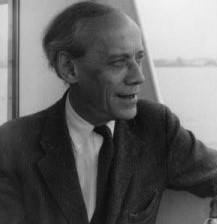
\includegraphics[width= 0.47\linewidth]{fig_Artin}
		\caption{\small\textit{\color{duongvaotoanhoc}Emil Artin}}
		\vspace*{-10pt}
	\end{figure}
	$\pmb{3.}$ \textbf{\color{duongvaotoanhoc}Từ dải bện đến lý thuyết nút}
	\vskip 0.1cm
	\textbf{\color{duongvaotoanhoc}Nút trong toán học là gì?}
	\vskip 0.1cm
	Một \textit{nút} trong toán học là một vòng dây khép kín (không có hai đầu, xem Hình $14$). Một \textit{cuộn dây gồm hai thành phần} được tạo bởi hai vòng dây khép kín (xem Hình $15$), một \textit{cuộn dây gồm ba thành phần} được tạo bởi ba vòng dây khép kín, v.v. \textit{Lý thuyết nút} là nhánh của tô--pô nghiên cứu các nút và các cuộn. Trong tô--pô, hình cầu không phân biệt với hình lập phương, còn cái bánh vòng và tách trà là một. Người ta không xét đến các thuộc tính như độ dài hay góc, mục đích là hiểu các tính chất bất biến đối với sự xoắn, kéo dãn hay nén.
	\begin{figure}[H]
		\vspace*{-10pt}
		\centering
		\captionsetup{labelformat= empty, justification=centering}
		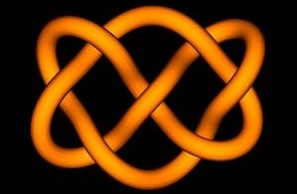
\includegraphics[width= 0.47\linewidth]{fig_14}
		\caption{\small\textit{\color{duongvaotoanhoc}Hình $14$. Một nút.}}
		\vspace*{-10pt}
	\end{figure}
	\begin{figure}[H]
		\vspace*{-10pt}
		\centering
		\captionsetup{labelformat= empty, justification=centering}
		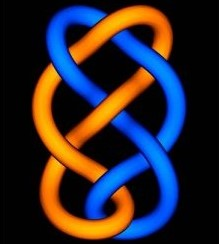
\includegraphics[width= 0.47\linewidth]{fig_15}
		\caption{\small\textit{\color{duongvaotoanhoc}Hình $15$. Một cuộn dây gồm hai thành phần.}}
		\vspace*{-10pt}
	\end{figure}
	Ngoài toán học, đặc biệt là tô--pô, lý thuyết nút có những ứng dụng trong các bài toán sinh học và hóa học. Chẳng hạn, nó được dùng trong nghiên cứu các phân tử đồng phân (có cùng công thức hóa học nhưng được sắp xếp khác nhau) hoặc trong nghiên cứu về tác động của một số enzyme đối với ADN.
	\vskip 0.1cm
	\textbf{\color{duongvaotoanhoc}Nguồn gốc của lý thuyết nút}
	\vskip 0.1cm
	Đóng góp đáng kể đầu tiên vào lý thuyết nút có lẽ là của Sir William Thomson (tức Kelvin) với thuyết ``xoáy nguyên tử" của ông. Năm $1867$, sau khi quan sát các vòng khói được tạo ra từ thí nghiệm của Peter Tait, nhà vật lý người Scotland, Thomson kết luận rằng các nguyên tử là những nút của ``những cuộn xoáy trong ê--te truyền ánh sáng". Theo đó, các nguyên tố hóa học ứng với các nút hoặc cuộn dây. Từ ý tưởng này, Peter Tait bắt đầu phân loại các nút, với niềm tin rằng ông đang tạo ra một bảng nguyên tố hóa học.
	\vskip 0.15cm
	\PIbox{
		\begin{figure}[H]
			\vspace*{-15pt}
			\centering
			\captionsetup{labelformat= empty, justification=centering}
			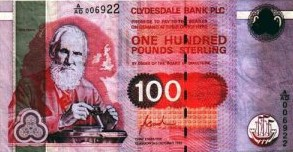
\includegraphics[width= 1\linewidth]{fig_William}
			\caption{\small\textit{\color{duongvaotoanhoc}William Thomson.}}
			\vspace*{-10pt}
		\end{figure}
		Sir William Thomson ($1824-1907$) là nhà vật lý học, nhà toán học và kỹ sư người Scotland. Ông được coi là một trong những nhà vật lý học hàng đầu của thế kỷ~$19$.
	}
	\vskip 0.1cm
	\textbf{\color{duongvaotoanhoc}Bài toán phân biệt hai nút}
	\vskip 0.1cm
	Bài toán trung tâm của lý thuyết nút là phân biệt, và xa hơn là phân loại, các nút. Phân biệt có nghĩa là quyết định xem liệu hai hình vẽ nút (hoặc cuộn dây) có biểu diễn cùng một nút (hoặc cuộn dây) hay không. Trong những năm $1920$, hai nhà toán học Mỹ Alexander và Briggs [$2$] và nhà toán học Đức Reidemeister [$16$], độc lập với nhau, đề xuất một thuật toán giải quyết một phần bài toán này. Thuật toán này có thể trả lời khẳng định nếu hai hình vẽ biểu diễn cùng một nút (hoặc cuộn), nhưng nó không trả lời trong trường hợp ngược lại. Nói cách khác, ta có thể nói hai nút giống nhau hay không, nhưng không thể nói hai nút có khác nhau hay không. Độc giả có thể cảm thấy điều này thật vô lý, nhưng nó là một nghịch lý thường thấy trong toán học. Hãy tưởng tượng bạn đang chờ ai đó. Bạn tự nhủ: ``Nếu cậu ấy đến, đó đúng là một người bạn." Nhưng nếu người đó không đến, bạn sẽ không biết đó có phải một người bạn hay không.
	\vskip 0.05cm
	Để phân biệt các nút, người ta sử dụng những cái mà các nhà toán học gọi là những \textit{bất biến}. Người ta gán cho mỗi hình vẽ cái nút một đối tượng (thường là một số hoặc một đa thức) chỉ phụ thuộc vào cái nút mà không phụ thuộc vào cách nó được vẽ. Nếu hai nút có những bất biến khác nhau thì chúng là hai nút khác nhau. Nếu không, ta chưa thể kết luận được gì.
	\vskip 0.1cm
	\textbf{\color{duongvaotoanhoc}Từ dải bện đến nút}
	\begin{figure}[H]
		\vspace*{-10pt}
		\centering
		\captionsetup{labelformat= empty, justification=centering}
		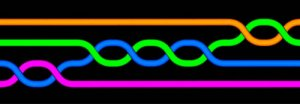
\includegraphics[width= 1\linewidth]{fig_16}
		\caption{\small\textit{\color{duongvaotoanhoc}Hình $16$. Dải bện đóng.}}
		\vspace*{-10pt}
	\end{figure}
	Từ một dải bện, ta có thể tạo ra một cuộn dây (hoặc một nút) bằng cách nối các đầu của dải bện với nhau, như minh họa trong Hình $16$. Một cuộn dây như vậy được gọi là một dải bện đóng. Alexander [$1$] đã chứng minh rằng mọi cuộn dây đều có thể được tạo ra theo cách này. Bạn đọc có thể thử với các thí dụ trong Hình $14$ và Hình $15$. Sau đó, Markov [$15$] đưa ra một thuật toán không hoàn toàn để xác định liệu hai dải bện cho trước có tạo thành cùng một cuộn dây (nhưng nó có thể không trả lời). Đây là hai kết quả cốt yếu để áp dụng lý thuyết bện vào các nút. Đặc biệt, chúng là điểm bắt đầu của sự đổi mới sâu sắc trong lý thuyết nút trong thập niên $1980$, với những công trình của Jones [$12$, $13$] và những bất biến được định nghĩa từ lý thuyết bện.
		\vskip 0.01cm
		\begin{tBox}
				\begin{wrapfigure}{l}{0.45\linewidth}
						\vspace*{-15pt}
						\centering
						\captionsetup{labelformat= empty, justification=centering}
						\hspace*{2pt}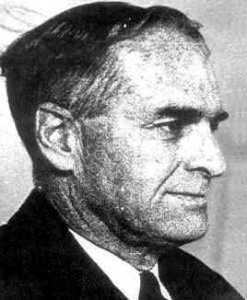
\includegraphics[width= 1.1\linewidth]{fig_Alexander}
						\caption{\small\textit{\color{duongvaotoanhoc}Alexander.}}
						\vspace*{-10pt}
					\end{wrapfigure}
				James W. Alexander ($1888-1971$) là một nhà toán học nổi tiếng người Mỹ. Là một trong những thành viên đầu tiên của Viện Nghiên cứu Cao cấp Princeton (từ $1933$ đến $1951$), ông đồng thời là giáo sư tại Đại học Princeton (từ $1920$ đến $1951$). Ông là một trong những người tiên phong của tô--pô đại số và lý thuyết nút. Ông cũng là một nhà leo núi cừ khôi, từng chinh phục được nhiều đỉnh cao. Về cuối đời, ông trở nên đơn độc và ẩn dật. Ông được biết đến như một người theo chủ nghĩa xã hội tích cực và danh tiếng của ông khiến ông bị chủ nghĩa MacCarthy để ý. Ông không xuất hiện trước công chúng kể từ năm $1954$, sau khi ký tên vào một bức thư ủng hộ Robert Oppenheimer.
			\end{tBox}
	
		\vspace*{-8pt}
		\begin{tBox}
				\begin{wrapfigure}{r}{0.4\linewidth}
						\vspace*{-15pt}
						\centering
						\captionsetup{labelformat= empty, justification=centering}
						\hspace*{-10pt}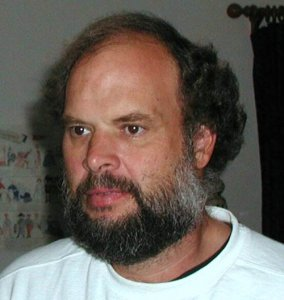
\includegraphics[width= 1.1\linewidth]{fig_Jones}
						\caption{\small\textit{\color{duongvaotoanhoc}Jones.}}
						\vspace*{-15pt}
					\end{wrapfigure}
				Vaughan F.R. Jones ($1952-2020$) là nhà toán học người New Zealand nổi tiếng với những công trình về các đại số von Neumann, các bất biến nút và lý thuyết trường bảo giác. Ông được trao Huy chương Fields năm $1990$ và là giáo sư ($1985-2011$) rồi giáo sư danh dự ($2011$ đến khi mất) tại Đại học California tại Berkeley. Các công trình của ông về bất biến nút dẫn tới những lời giải bất ngờ cho nhiều bài toán cổ điển trong lý thuyết nút và tô--pô thấp chiều.
			\end{tBox}
	\textbf{\color{duongvaotoanhoc}Tài liệu tham khảo}
	\vskip 0.1cm
	{\small[$1$] J.W. Alexander. \textit{Deformations of an n-cell}. Proc. Nat. Acad. Sci. USA $9$ ($1923$), $406-407$.
	\vskip 0.1cm
	[$2$] J. W. Alexander, G. B. Briggs. \textit{On types of knotted curves}. Ann. of Math. ($2$) $28$ ($1926/27$), no. $1-4$, $562-586$.
	\vskip 0.1cm
	[$4$] E. Artin. \textit{Theorie de Zöpfe}. Abhandlungen Hamburg $4$ ($1925$), $47-72$.
	\vskip 0.1cm
	[$12$] V.F.R. Jones. \textit{A polynomial invariant for knots via von Neumann algebras}. Bull. Amer. Math. Soc. (N.S.) $12$ ($1985$), no. $1$, $103-111$.
	\vskip 0.1cm
	[$13$] V.F.R. Jones. \textit{Hecke algebra representations of braid groups and link polynomials}. Ann. of Math. ($2$) $126$ ($1987$), no. $2$, $335-388$.
	\vskip 0.1cm
	[$15$] A. Markoff. \textit{Fundations of the algebraic theory of tresses}. Trav. Inst. Math. Stekloff $16$ ($1945$).
	\vskip 0.1cm
	[$16$] K. Reidemeister. \textit{Elementare Begründang der Knotentheorie}. Abh. Math. Sem. Univ. Hamburg $5$ ($1926$), $24-32$.}
\end{multicols}